\documentclass[10pt]{article}
\usepackage[polish]{babel}
\usepackage[utf8]{inputenc}
\usepackage[T1]{fontenc}
\usepackage{amsmath}
\usepackage{amsfonts}
\usepackage{amssymb}
\usepackage[version=4]{mhchem}
\usepackage{stmaryrd}
\usepackage{graphicx}
\usepackage[export]{adjustbox}
\graphicspath{ {./images/} }

\title{GIMNAZJUM }

\author{}
\date{}


\begin{document}
\maketitle
\begin{enumerate}
  \item Przekątne trapezu \(A B C D\) są prostopadłe i przecinają się w punkcie \(E\). Wiadomo, że \(C D=13, C E=5\) oraz \(B D=30\). lle wynosi pole trójkąta \(A C D\) ?
  \item W turnieju tenisowym rozgrywanym systemem pucharowym wystartowało 2017 zawodników. W każdej rundzie losowane są pary zawodników, którzy grają ze sobą. Zwycięzca pojedynku przechodzi do\\
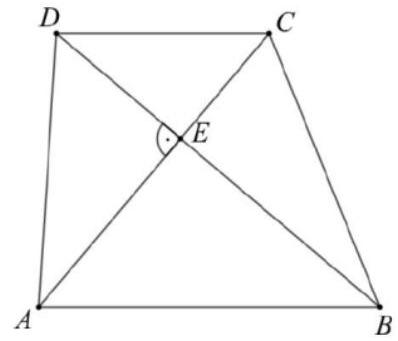
\includegraphics[max width=\textwidth, center]{2024_11_21_ea6946dc5e9ed6632317g-1}\\
kolejnej rundy (nie ma remisów). Jeśli liczba zawodników w danej rundzie jest nieparzysta, jeden zawodnik przechodzi do kolejnej rundy bez rozgrywania pojedynku. Ile spotkań trzeba rozegrać, aby wyłonić zwycięzcę?
  \item Iloma cyframi będzie zapisana liczba uzyskana jako wynik działania \(125^{21} \cdot 4^{32}\) ?
\end{enumerate}

\section*{LICEUM}
\begin{enumerate}
  \item Rozwiąż układ równań
\end{enumerate}

\[
\left\{\begin{array}{l}
x^{2}+3 y^{2}=1 \\
(x+3 y)^{2}=1
\end{array}\right.
\]

\begin{enumerate}
  \setcounter{enumi}{1}
  \item Podaj największy dzielnik liczby \(10^{10}\), który w zapisie dziesiętnym nie zawiera cyfry 0.
  \item W trójkącie prostokątnym \(A B C\) poprowadzono wysokość \(C D\) z wierzchołka kąta prostego. Okrąg, którego średnicą jest wysokość \(C D\), odcina na przyprostokątnych trójkąta odcinki długości \(k\) i \(l\). Oblicz pole trójkąta \(A B C\).
\end{enumerate}

\end{document}